\documentclass[tikz, border=3mm]{standalone}
\usepackage{tikz}
\usetikzlibrary{
    arrows.meta,         % For arrow tips
    decorations.markings,% For placing arrows along paths
    calc,                % For coordinate calculations
    positioning          % For label positioning
}

\begin{document}
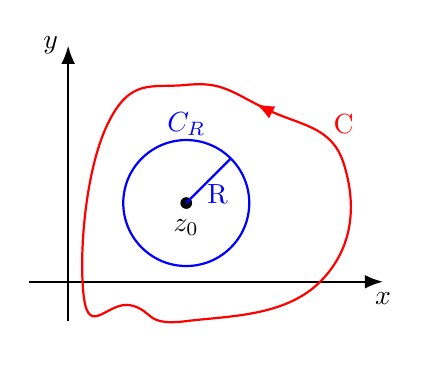
\begin{tikzpicture}[
    >=Latex, % Set default arrow tip style
    axis/.style={->, thick}, % Style for axes
    curve/.style={thick},    % Base style for curves
    dot/.style={fill=black, circle, inner sep=1.5pt},
    labelstyle/.style={}, %
         midarrow/.style={
        decoration={markings, mark=at position 0.5 with {\arrow{Latex[length=2mm]}}},
        postaction={decorate}
    },
    midarrowL/.style={
        decoration={markings, mark=at position 0.2 with {\arrowreversed{Latex}}},
        postaction={decorate}
    }]

% #1=pos, #2=color, #3=tip(> or <)
 % Style for placing an arrow on a path
    % Axes
    \draw[axis] (-0.5, 0) -- (4, 0) node[below] {$x$};
    \draw[axis] (0, -0.5) -- (0, 3) node[left] {$y$};

    % Define center and radius for inner circle
    \coordinate (z0) at (1.5, 1.0);
    \def\radius{0.8};

    % Draw Inner Blue Circle (CR)
    \draw[curve, blue] (z0) circle (\radius);
    \node[blue] at ($(z0)+(90:\radius+0.2)$) {$C_R$}; % Label CR above circle

    % Draw Center Point z0
    \node[dot, label={[labelstyle, black]below:$z_0$}] at (z0) {};

    % Draw Radius Line and Label R
    \coordinate (R_end) at ($(z0)+(45:\radius)$); % Endpoint on circle at 45 deg
    \draw[blue, thick] (z0) -- (R_end);
    \node[blue, below=1pt] at ($(z0)!0.7!(R_end)$) {R}; % Label R along the line

    % Define coordinates for outer blob C (adjust as needed)
    

    % Draw Outer Red Blob (C) with CCW Arrow
    % Arrow at pos 0.6, red, pointing < (CCW)
    \draw[curve, red, midarrowL] plot [smooth cycle, tension=0.8] coordinates {
(0.2, -0.2)
        (0.5, 2.0)
        (1.5, 2.5)
        (2.5, 2.2)
        (3.5, 1.5)
        (3.2, 0.0)
        (1.5, -0.5)
        (0.8, -0.3)};
    \node[red] at (3.5, 2.0) {C}; % Label C

\end{tikzpicture}
\end{document}